\documentclass[12pt,floatfix,showpacs]{revtex4-1}

\usepackage{amssymb,amsmath,amsfonts}
\usepackage{graphicx}
\usepackage{subfig}

\newcommand{\eg}{\emph{e.g., }}
\newcommand{\ie}{\emph{i.e., }}
\newcommand{\etal}{\emph{et al.}}

% remove these for final publication 
\usepackage{color} 
\newcommand{\note}[1]{\textcolor{red}{#1}}
\newcommand{\gnote}[1]{\marginpar{\textcolor{red}{\scriptsize{#1}}}}

\graphicspath{{./graphics/}}

\begin{document}

\title{Eqtools: Modular, Extensible, Open-Source, Cross-Machine Python Tools for Working with Magnetic Equilibria}

\author{M. A. Chilenski}
\email[]{markchil@psfc.mit.edu}
\affiliation{MIT Plasma Science and Fusion Center}

\author{I. C. Faust}
\affiliation{MIT Plasma Science and Fusion Center}

\author{J. R. Walk}
\affiliation{MIT Plasma Science and Fusion Center}

\date{\today}

\begin{abstract}
 An introduction to the eqtools package, a modular, extensible, open-source toolkit in the Python programming language for handling magnetic equilibria from tokamaks, is presented.  The eqtools package provides a single interface for working with magnetic equilibrium data, both for handling derived-quantity data and mapping between coordinate systems in the flux grid, extensible to function with data from different experiments, data formats, and magnetic-reconstruction codes, replacing the static solutions currently used on tokamak experiments.  Moreover, the development of magnetic-equilibrium functionality in the Python language removes a substantial barrier to code migration and new development in Python, which presents a number of attractive advantages.  In this paper, we introduce the modular structure and design of the eqtools package and detail the workflow for usage and expansion to additional devices.  The implementation of a novel three-dimensional spline solution (in two spatial coordinates and in time) for improved timebase accuracy is also detailed.  Finally, Benchmarking for accuracy and speed against existing methods are detailed.
\end{abstract}
\gnote{other PACs numbers?}

\pacs{52.55.Fa}

\maketitle

%%%%%%%%%%%%%%%%%%%%%%%%%%%%%%%%%%%%%%%%%%%%%%%%%%%%%%%%%%%%

\section{Introduction}\label{sec:intro}

The basic computational tasks associated with magnetic-equilibrium reconstructions -- namely, the handling of derived quantities (\eg calculated plasma current, safety-factor profiles) and the mapping between real-space and flux coordinate systems for experimental data -- are universal among tokamak experiments.  Despite this commonality, experiments typically utilize in-house solutions developed for the particulars of that experiment's data storage and usage.  This ad-hoc development of base-level functionality inhibits the mobility of higher-level codes to other devices (as the code may require substantial modification to address the particulars of the new data storage design).  Moreover, such development is often quite static, such that the implementation is difficult to extend to new data formats (for example, to handle both a primary MDSplus-based data storage system \note{cite?} and the \emph{eqdsk} storage files produced directly by the EFIT reconstruction code \cite{Lao1985}), necessitating parallel workflows for functionally identical tasks depending on the data source.  Best design practices call for the vagaries of data source and storage implementation to be placed in the back end, presenting a consistent, straightforward interface common between machines and code implementations to the research scientist.

The new \emph{eqtools} package provides a modular, extensible, cross-machine toolkit developed in the Python programming language for handling magnetic-equilibrium data.  The \emph{eqtools} package provides a consistent \& straightforward interface to the researcher for both coordinate-mapping routines (which are historically handled in separate standalone routines) and derived-quantity data handling (which are often handled with manual hooks into data storage).  Moreover, \emph{eqtools} is constructed in a modular, object-oriented design, such that the package is easily extensible to handle data from different experiments and reconstruction codes, allowing the researcher a single unified interface for data from any machine or code.  The implementation of reconstructed-equilibrium handling in the Python language removes a substantial barrier to the adoption of Python as a day-to-day working language for tokamak research, which offers numerous advantages in ease of use, computational speed, user/developer base, and free \& open-source implementations compared to current common working languages for fusion research.\gnote{where to point to github?}

This paper details the design and implementation of the eqtools package, particularly the paradigm for extension to new machines (section \ref{sec:design}), describes the implementation of a trivariate spline method for improved coordinate-mapping accuracy in the time dimension (section \ref{sec:trispline}), and presents runtime and accuracy benchmarks against the current IDL implementation at Alcator C-Mod (section \ref{sec:benchmark}).

\section{Package Design and Use}\label{sec:design}

The \emph{eqtools} package is designed to present a consistent, human-readable interface to the user for both data handling of derived quantities and mapping routines between coordinate systems, all contained within a single persistent object (herein referenced in code snippets as \verb|eq|).  For example, Pulling the calculated value for the poloidal flux on-axis, $\psi_0$, is simply \verb|eq.getFluxAxis()| -- this replaces arrangements that may involve manual hooks into the data system (as is the case at Alcator C-Mod) and interaction with non-intuitive internal variable names (as is the case with EFIT outputs\gnote{too harsh?}).  Similarly, mapping routines are handled internally in the \verb|eq| object -- mapping from the machine RZ grid to normalized poloidal flux, for example, is simply \verb|eq.rz2psinorm(R,Z,t,...)|.  One notable consequence of this is that intermediate spline calculations for the mapping routines are stored in the persistent object -- compared to typical standalone mapping routines (which must start from scratch for each function call) this allows substantial speed gains for subsequent mapping calculations with the same equilibrium object.

The \emph{eqtools} package is structured such that the user-facing methods (for data pulls or mapping routines) are consistent between implementations for different machines or reconstruction codes, and moreover that the creation of new implementations (for new machines or codes) requires minimal new code.  This inheritance structure is depicted in figure \ref{fig:flowchart}.  The base level of the inheritance structure (shown in blue in figure \ref{fig:flowchart}) provides the abstract class \verb|Equilibrium| -- this defines the skeleton structure for the data system (ensuring that child classes use a consistent format) and defines the mapping routines, which are inherited and used by each child class.  The methods therein are sufficiently general to be used by any grid-based equilibrium reconstruction.

\begin{figure}[p]
 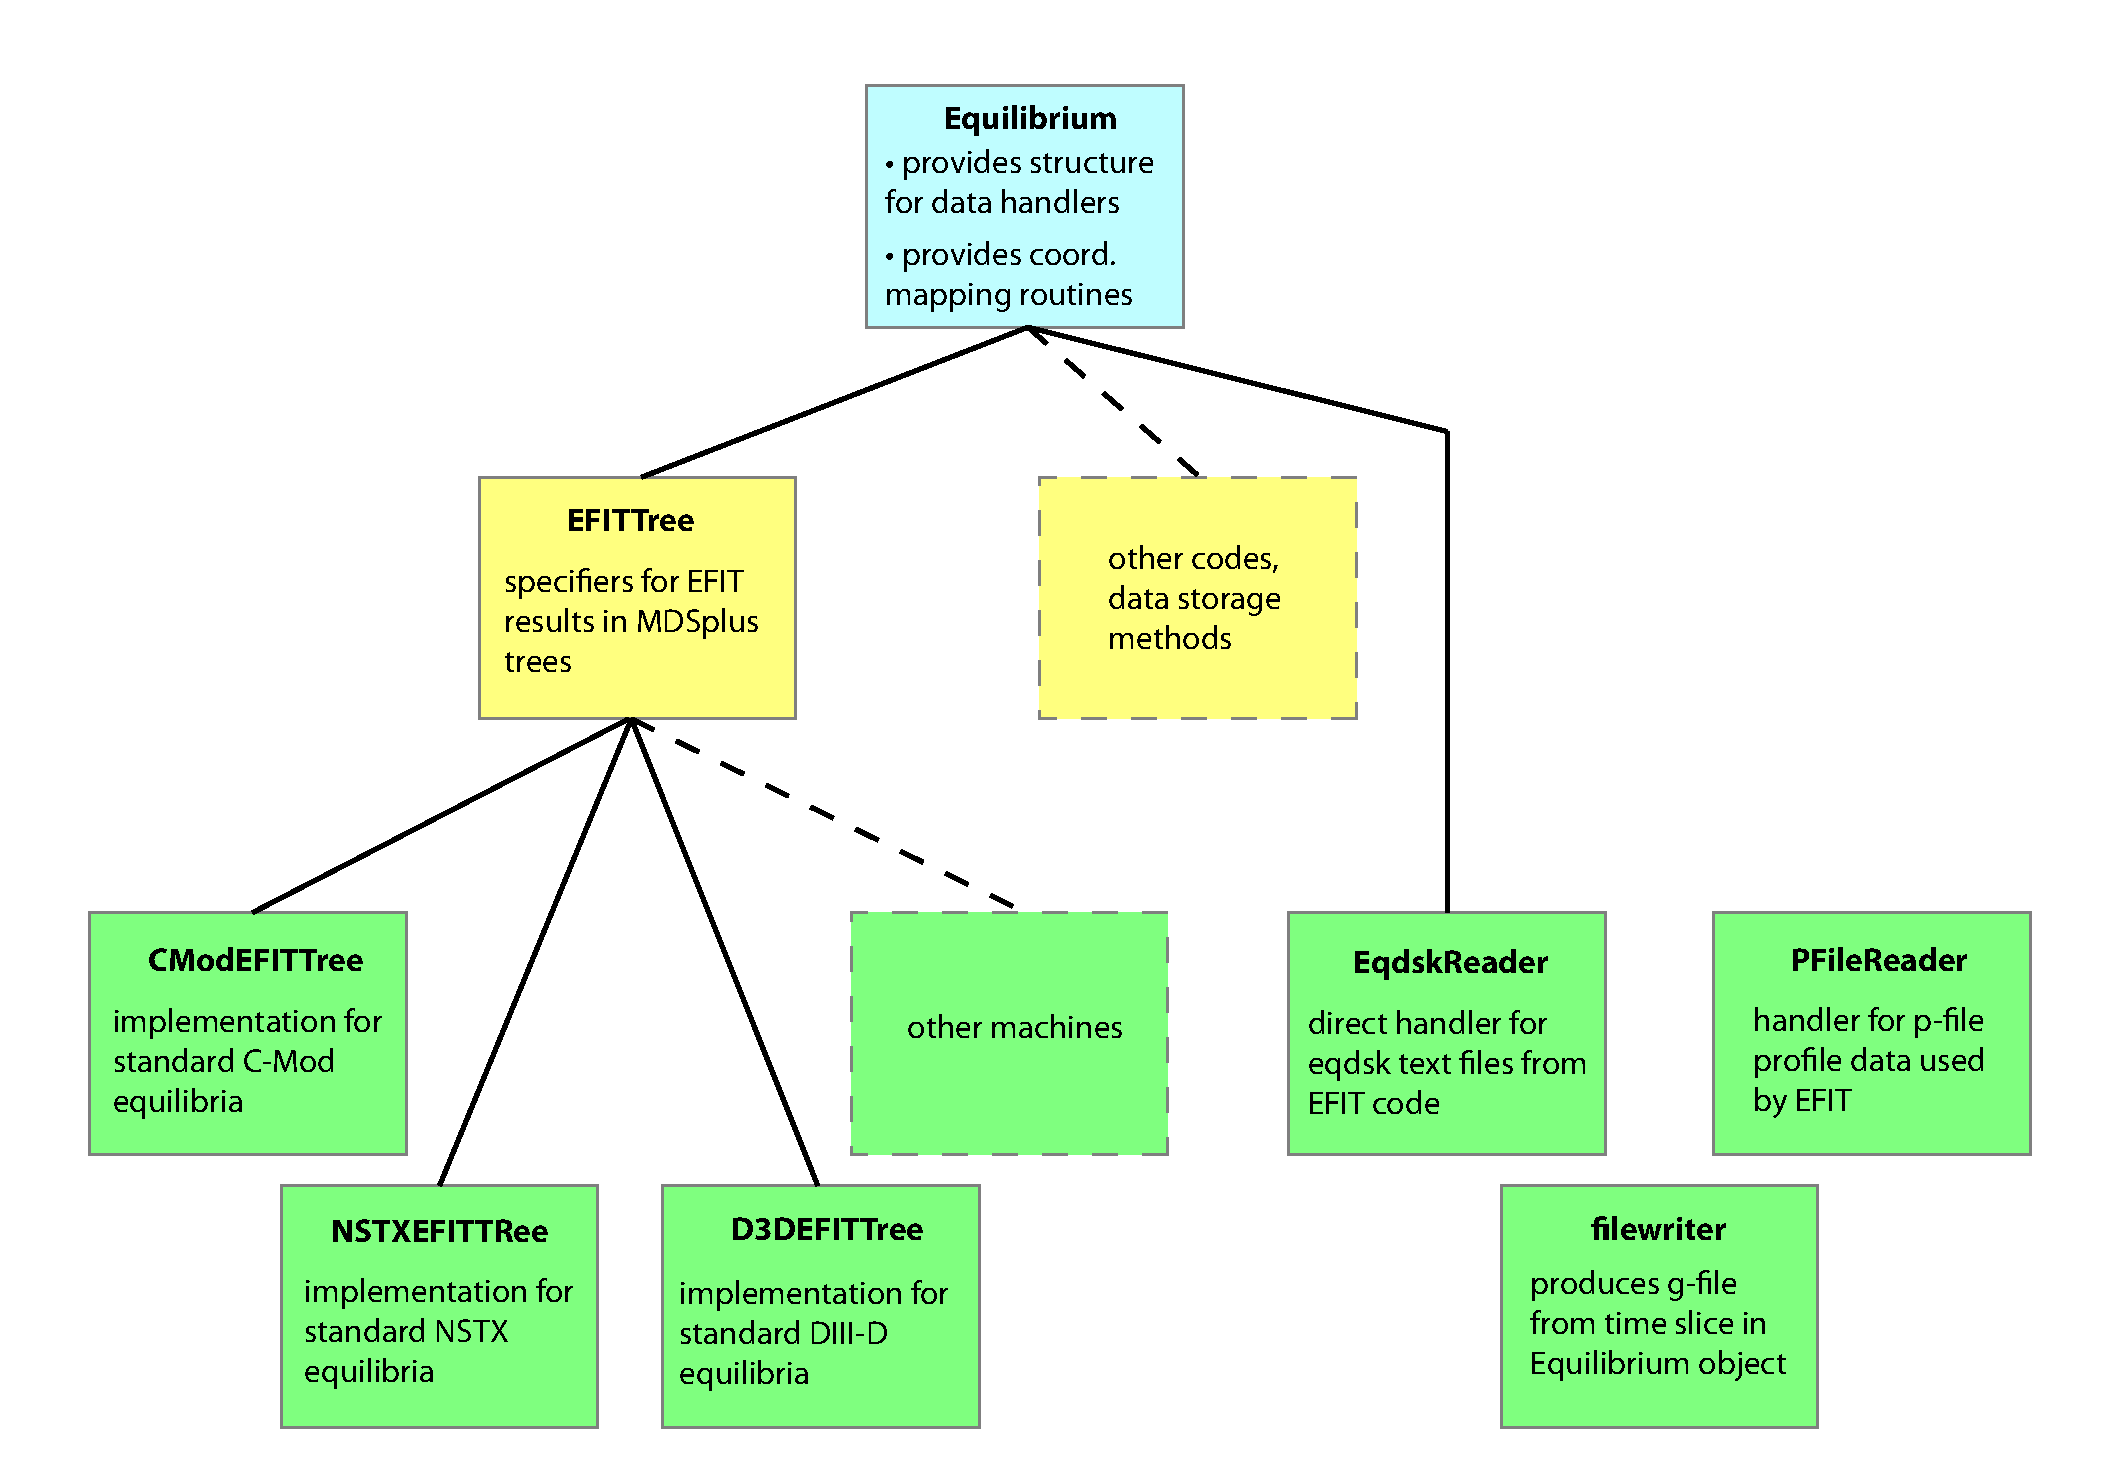
\includegraphics[width=\textwidth]{graphics/flowchart.pdf}
 \caption{Inheritance schematic for the \emph{eqtools} package.  The base abstract class (blue) provides a skeleton structure for the derived-data handlers, as well as providing the complete set of coordinate-mapping routines.  Intermediate abstract classes (yellow) prescribe the handling for data storage systems and codes -- at present the relatively-ubiquitous EFIT reconstruction stored in MDSplus tree structures is provided.  User-facing classes (green) handle the details of machine-specific implementations.  Dashed lines denote classes that have not yet been implemented, but which can be introduced into the package in a straightforward manner due to its modular construction.  The user interface is consistent, as it is provided by the parent classes -- code migration between machines requires only changing which child class is called for the reconstruction.  The \emph{EqdskReader} class, which directly handles \emph{eqdsk} text files from EFIT, inherits directly from the base class as it is sufficiently unique to not warrant an intermediate abstract class.  \note{add filewriter?}}
 \label{fig:flowchart}
\end{figure}

An intermediate inheritance level (shown in yellow in figure \ref{fig:flowchart}) provides more specific methodology (while still maintaining cross-machine generality) -- for example, the \verb|EFITTree| class provides methods for EFIT reconstructions stored in MDSplus tree structures (as is used on C-Mod, NSTX, and DIII-D\gnote{cites?}).  This minimizes the need for repeated code in machine-specific versions of common code implementations.  The user-facing inheritance level (shown in green in figure \ref{fig:flowchart}) finalizes the specific details of implementation for a given reconstruction code, data-storage methodology, and machine implementation (\eg \verb|CModEFITTree|, \verb|NSTXEFITTree|, \verb|D3DEFITTree|).  These user-facing implementations typically differ by relatively little code (on the order of 100 lines in the case of \verb|CModEFITTree| and \verb|NSTXEFITTree|), and extension modules to the code can be quickly developed in most cases.\gnote{check line count}

In addition to the already-developed modules inheriting \verb|EFITTree|, the code current contains the \verb|EqdskReader| module, which directly interfaces with the \emph{eqdsk} text files (specifically, the ``g-file'' and ``a-file'' containers, which store equilibrium and scalar derived-quantity data, respectively) generated by EFIT.\gnote{cite?}  This allows a single unified interface for both the tree-based and portable text-file data storage common to US experiments.\gnote{expand?  other countries?}  Due to the unique structure of the code necessary to read text-file data (which is done directly in \verb|EqdskReader|), \verb|EqdskReader| directly inherits mapping routines and skeletal structure from \verb|Equilibrium|, without an intermediate stage; however, as new text-file-based storage methods are implemented in \emph{eqtools} sufficient commonality may be found to necessitate the creation of a intermediate abstraction level for generalized text-file storage systems in subsequent versions of the \emph{eqtools} package.

In addition to the \verb|EqdskReader| module, which handles equilibrium and derived-quantity data from g- and a-file outputs from EFIT, the \emph{eqtools} package provides a \verb|PFileReader| object to handle plasma-profile data from the ``p-files'' associated with EFIT.  While this does not require access to the reconstructed equilibrium (and thus is separate from the \verb|Equilibrium| inheritance structure) profile data is commonly paired with the reconstructed equilibrium -- as such, the \emph{eqtools} package provides a built-in methodology to handle the additional data.  The \emph{eqtools} package also contains a package-level method, \verb|filewriter|\gnote{check naming!} to produce g-files from classes in the \verb|Equilibrium| inheritance tree, allowing easy generation of portable datasets from the main data-storage method.\gnote{reword?}

\section{Tri-Spline Implementation}\label{sec:trispline}

Sets of equilibria create time histories which are often generated at different times and at different rates from other plasma measurements. Parameters based off of these sets will suffer from discontinuties introduced by the equilibria when sampled at higher rates than that of the set.  When the set of equilibria achieves the nyquist frequency for variations of interest, an additional interpolation in time can accurately remove aliasing errors induced by the timebase mismatch. The additional temporal dimension requires the use of higher dimensional interpolators, of which a fast tricubic interpolation scheme was developed. 

The additional time dimension and subsequent higher-dimensionality increases the evaluation time of the mapping routines. A tricubic interpolating spline is used to evaluate the three-dimensional flux grid. The time dimension is assumed to be rectilinear in nature with respect to the spatial dimensions, allowing for the use of developed optimized matrix methods for extracting the coefficients of a tricubic interpolating spline \note{quote Leiken here}. The higher dimensionality of the problem scales the necessary computational time similarly due to the increased necessary information (x64 increase in matrix computation). Other non-three-dimensional parameters also require further computation due to the inherent complication of increasing the number of dimensions. While use of persistence of the coefficients can achieve similar times when subject to calculations in the same `voxel', the overall computation is slower when compared to lower-dimensional mapping.

Significant time savings can be recovered for tricubic interpolation computation when the data grid is regular, which is often the case for sets of magnetic equilbria. Recovering the spline coefficients requires the calculation of a number of derivatives in each dimension, which for a regular grid can be achieved with finite difference matrix $\boldsymbol{B}$. The new \emph{a priori} inclusion of $\boldsymbol{B}$ in the spline calcuation matrix $\boldsymbol{A_{inv}}$ removes the necessary derivative generation and reduces total computation by half (denoted 
$\boldsymbol{A_{inv}^*}$) . This calculation requires a collection of the nearest 4x4x4 grid of points to the point of interest $\boldsymbol{x}$ to extract spline coefficents $\boldsymbol{y}$.

\begin{equation}
\boldsymbol{y} = \boldsymbol{A_{inv}} ( \boldsymbol{B} \boldsymbol{x}) = \boldsymbol{A_{inv}^*}\boldsymbol{x}
\end{equation}
Where
\begin{equation}
\boldsymbol{A_{inv}^*} = \boldsymbol{A_{inv}}\boldsymbol{B} 
\end{equation}

The code for all of the tricubic spline interpolation was written in C and was integrated into python using the F2PY \note{quote f2py paper here} pacakge. Other programming languages and codes with sufficienct C APIs can access the optimized trispline code for use outside of magnetic reconstructions, and is well contained in accepting 3 dimensional data for analysis.





\section{Benchmarking}\label{sec:benchmark}

\begin{figure}[ht]
 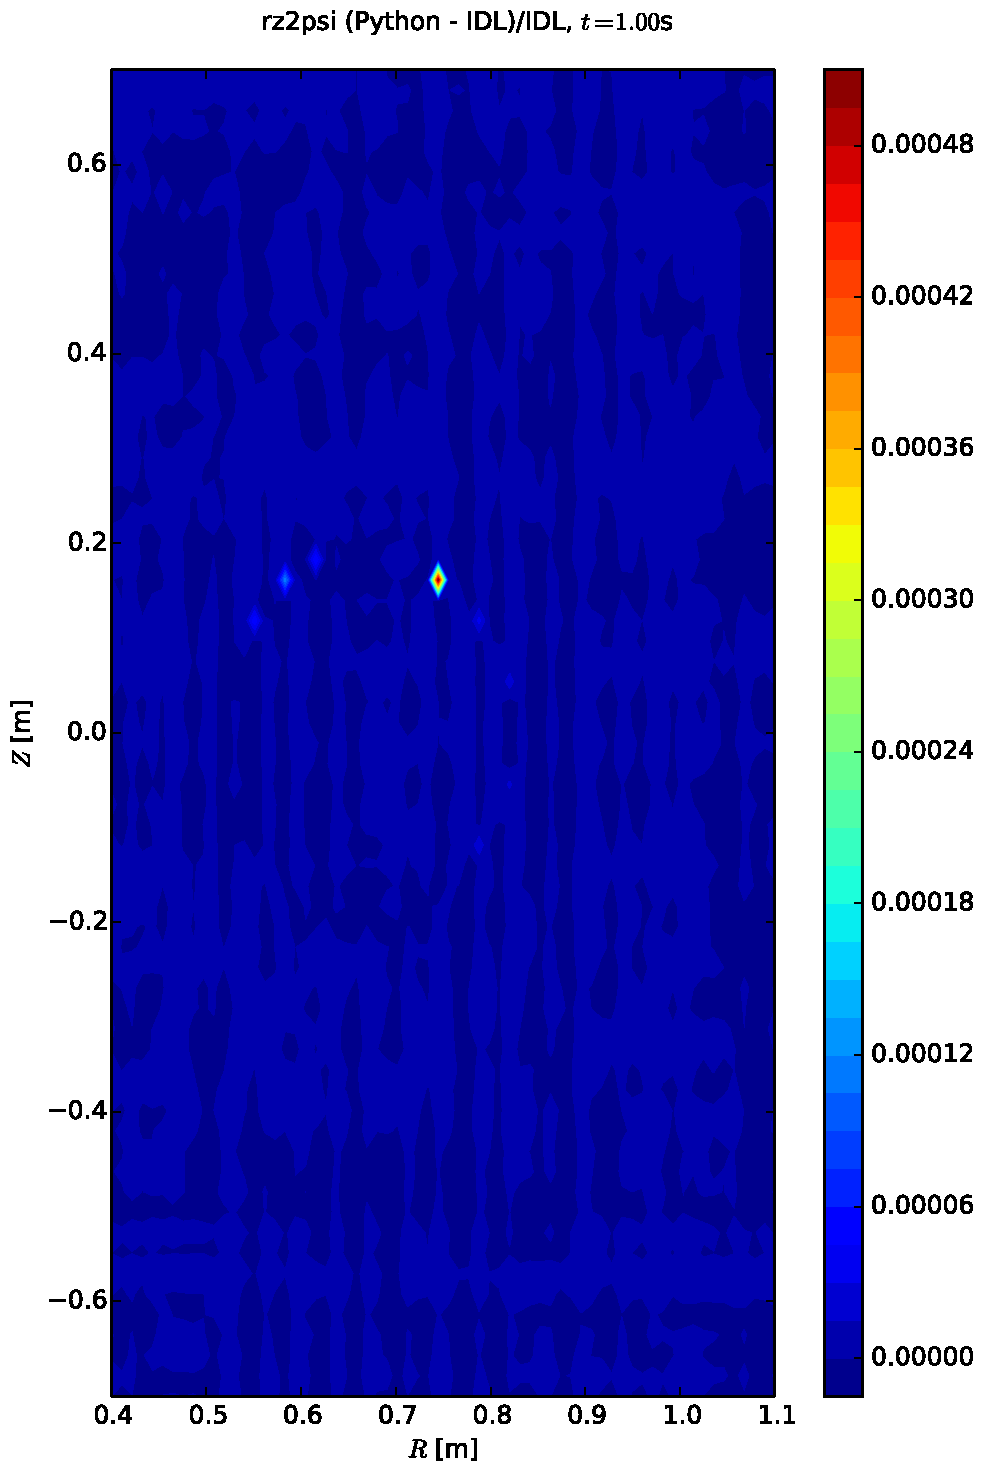
\includegraphics[width=0.5\textwidth]{graphics/RZ2psi_rel_diff.pdf}
 \caption{Relative difference between calculations of a mapping between the RZ grid and poloidal flux for the \emph{eqtools} and the current IDL implementation of the mapping routine for an example Alcator C-Mod reconstructed equilibrium.  Relative differences of less than half a percent are typical.  \note{source of diff?  EFIT, spline error?  pair with flux map of equilibrium for comparison?}}
 \label{fig:rz2psi_diff}
\end{figure}

\section{Summary}\label{sec:summary}

%%%%%%%%%%%%%%%%%%%%%%%%%%%%%%%%%%%%%%%%%%%%%%%%%%%%%%%%%%%%

\begin{acknowledgements}
 acknowledgements go here.
\end{acknowledgements}

\bibliographystyle{aipnum4-1}
\bibliography{eqtools_paper}

\end{document}
